Nesse capítulo serão apresentados detalhes da implementação realizada nesse trabalho. O código foi desenvolvido em python com auxílio da biblioteca PETSc (\citet{petsc-user-ref}). O PETSc é uma biblioteca famosa com diversas rotinas para computação científica, possui paralelismo utilizando MPI, estruturas de dados para matrizes esparsas, métodos de Krylov para solução de sistemas lineares, conjunto de pré-condicionadores (em particular os ILU), dentre outros. Estudos da performance do PETSc podem ser encontrados \citet{petsc-efficient}. Utilizar o PETSc junto com o python é possível através do \textit{bindings} realizados pelo petsc4py (\citet{Dalcin2011}). O código aqui apresentado foi desenvolvido em sequencial. 



\section{Estrutura de Classes}

Primeiramente, foi necessário desenvolver uma estrutura para resolver problemas através do método dos elementos finitos para depois iniciar implementação com o método multiescala. Para esse desenvolvimento três principais classes foram implementadas: Element, Node, FemContext. As responsabilidades das classes são descritas abaixo:

\begin{itemize}
    \item \textbf{Node}: essa classe tem como intuito representar os nós do problema de elementos finitos. Guarda como propriedade as coordenadas x, y correspondentes, uma numeração global associada ao grid fino e se o nó pertence ou não a uma fronteira com condição de Dirichlet.
    \item \textbf{Element}: essa classe tem como intuito representar os elementos do problema de elementos finitos. Tem uma referência para os nós que pertencem ao elemento. Guarda os valores do coeficiente de Young e Poisson. Sabe calcular as funções de forma em coordenadas locais conforme \eqref{eq:definicaofuncform}. Assim, é responsável por calcular a matriz do elemento local.
    \item \textbf{FemContext}: essa classe tem como intuito representar um problema de elementos finitos. Ela possui o conjunto de elementos e nós do problema em questão. Dá a numeração de cada um dos graus de liberdade dos nós. Calcula a matriz de rigidez através do algoritmo apresentado no Capítulo \ref{ch:discretizacao} e o lado direito correspondente. 
\end{itemize}

Essas três classes são capazes de realizar a solução de um problema de elementos finitos. Existem métodos auxiliares para ler dados de entrada para montar os elementos e nós de um grid fino. Um fato importante é que a classe \textbf{FemContext} é que tem a numeração dos graus de liberdade, isso acontece, pois, para calcular a base de diferentes problemas locais de elementos finitos serão resolvidos e essa classe será reaproveitada. Em uma implementação de elementos finitos clássica o mais natural seria a numeração do grau de liberdade está associada com um nó.


Para a implementação do método multiescala, foi adicionada criada a classe \textbf{Multiscale}, essa classe tem como responsabilidade receber um objeto \textbf{FemContext} que representa o grid fino e calcular os operadores de prolongamento ($\mathbf{P}$), restrição ($\mathbf{P}^T$) e operador grosso ($\rigidmatrixcoarse$).


\section{Montagem dos Operador Multiescala}

O primeiro passo para utilizar o método multiescala é a escolha do nível de engrossamento. A implementação aceita diferentes fatores para a direção x e y, apesar dos testes serem apresentados com o mesmo fator. O método \textbf{CoarseContext} é responsável por realizar a tarefa de construir $\mathbf{P}$ e $\rigidmatrixcoarse$. Essa tarefa é dividida nos seguintes passos: 

\begin{itemize}
    \item Criar objetos \textbf{FemContext} para cada um dos problemas locais.
    \item Adicionar os nós e elementos correspondentes em cada um dos seus respectivos \textbf{FemContext}
    \item Para cada \textbf{FemContext} calcular a matriz de rigidez $\rigidmatrixelementms$.
    \item Resolver os oito problemas associados as funções de Base.
    \item Fazer o Assembly do operador de prolongamento.
    \item Calcular $\rigidmatrixcoarse = \mathbf{P}^T \rigidmatrix \mathbf{P}$
\end{itemize}

A Figura \ref{fig:esquemaconstrucao} apresenta um esboço da construção desse operador. Pode-se perceber que os problemas são independentes exceto pela solução dos problemas das arestas em comum. A implementação desse trabalho resolveu esse mesmo problema na fronteira duas vezes, uma vez em cada problema local diferente, uma implementação mais otimizada pode resolver apenas uma vez cada problema de fronteira.

\begin{figure}[!htbp]
\centering
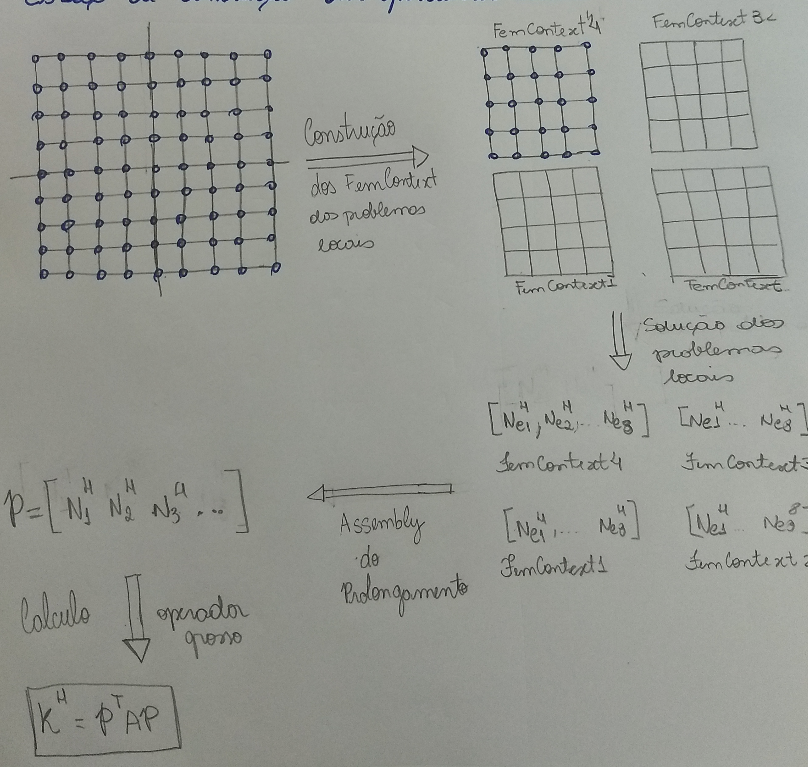
\includegraphics[width=\textwidth]{chap07/figs/esquemaprolongamento.png}
\caption{Esquema de construção dos operadores grossos.}
\label{fig:esquemaconstrucao}
\end{figure}

O cálculo das matrizes dos operadores locais  $\rigidmatrixelementms$ tem os mesmos coeficientes presentes na matriz de rigidez $\rigidmatrix$ visto que o operador de \eqref{eq:edp_geomec} é o mesmo de \eqref{eq:operadorlocal}. Dessa forma, a matriz de um operador local é uma submatriz do operador original, portanto, foi utilizado o método GetSubMatrix das matrizes do petsc para construir $\rigidmatrixelementms$ a partir de $\rigidmatrix$.


A classe \textbf{Multiscale} também possui um método solve, que só pode ser chamado a após o método \textbf{CoarseContext} ter sido executado. Esse método recebe como entrada um vetor $\mathbf{f}^h$ relacionado a um lado direito do grid fino e resolve o problema no grid grosso e retorna para o grid fino. Em outras palavras, esse método retorna o seguinte valor $\mathbf{P}(\rigidmatrixcoarse)^{-1}\mathbf{P}^T \mathbf{f}^h$. Esse método será aplicado ao resíduo quando o multiescala estiver sendo utilizado como pré-condicionador nos estudos aqui apresentados. 
                                                                                       